% 当前实现。每页回答一个具体的源码阅读问题。
\clearpage
\begingroup
\setlength{\parskip}{8pt}
\section{场景、设备与绘制命令}\label{sec:ownership}
把 Sponza 切换到环境遮蔽视图，原本有颜色的柱面变成了灰白色。再用鼠标点它，选中的仍是同一个建筑实体。场景面板保留着一张记载物体编号的图，而屏幕上显示哪种颜色，由用户选的光照效果决定。两份结果在图中分别走左、右两条路。

\figpanel{scene-compute}{从上往下读。箭头表示上一行调用下一行。左列画出颜色与物体编号，右列根据模型和灯光计算显示颜色。编辑器在帧末选一张颜色图交给 ImGui。}

\code{SceneRenderer::DrawGeometry} 遍历场景组件，取得网格、材质、变换和实体编号。它选好这次要画的东西，把一次索引绘制交给 \code{CommandList::DrawIndexed}。网格创建发生得更早。加载器把顶点和索引交给 \code{RenderDevice::CreateMesh}，以后移动相机只需改变传给绘制命令的矩阵。

光照视图还需要读场景里的点光源。\code{LightingPreview} 根据编辑器的开关组合直接光、间接光和屏幕效果。算法把输入和工作组数量交给 \code{ComputeDevice::Dispatch}。工作组就是一批一起运行着色器的调用，例如最终显示程序每组覆盖 $8\times8$ 个像素。Vulkan 将工作记下并提交给队列，等计算完成，面板就能读这张图。即使把右列的 GTAO 换成屏幕反射，左列在鼠标处留下的实体编号仍然有效。
\readings{\path{RedflagForge/src/LightingPreview.cpp}\quad
\path{Redflag/src/Redflag/Renderer/SceneRenderer.cpp}\quad
\path{Redflag/src/Redflag/Renderer/RHI/}}

\clearpage
\section{贴图的持有与释放}\label{sec:ownership-texture}
给两面墙各配一份材质，两份材质都可以保存同一张砖墙贴图。项目用 \code{Ref<T>} 表示共同持有对象，它是 C++ 的 \code{std::shared\_ptr<T>}。复制材质中的这份引用，只增加一个持有者。两面墙都用得上的那些纹理像素在显存里仍然只有一份。

在 Vulkan 后端，一张材质贴图内部单独持有一幅 \code{Image}。这里用 \code{Scope<Image>}，也就是 \code{std::unique\_ptr<Image>}。它只能有一个所有者，移动它可以交出所有权。贴图另外用 \code{Ref<TexturePool>} 留住登记这张纹理的池，因而归还登记项时，池一定还在。两个类型都能用箭头访问成员，读源码时可以先看声明，分清这一步是在借用、独占，还是共享。
\codewhere{源码}{Redflag/src/Platform/Vulkan/VulkanDrawResources.cpp}{Image 析构函数}
\begin{lstlisting}
Image::~Image()
{
(*@\rhicomment{// 先销毁引用图像的视图，最后归还显存。}@*)
    vkDestroyImageView(Device, View, nullptr);
    vkDestroyImage(Device, Handle, nullptr);
    vkFreeMemory(Device, Memory, nullptr);
}
\end{lstlisting}

着色器通过图像视图访问像素，图像又依赖分配给它的显存。所以这三次调用沿着依赖反方向释放。C++ 在对象生命结束时调用析构函数，将归还资源这件事放进对象本身，这就是 RAII。材质继续保存引用时图像仍然有效。后端还须安排 GPU 完成时间，下一页会用一次面板换图说明。

\termaside{编辑器通过 \code{RenderDevice::SetCurrent(m\_Draw.get())} 登记当前设备。\code{get()} 返回一个可以访问对象的普通指针，设备仍由编辑层的 \code{Scope<VulkanDraw>} 独占。退出时先解除登记，再销毁它。}{读代码时留意的区别}{函数参数 \code{const Ref<T>\&} 借用调用者的智能指针。函数若把它复制进成员或数组，那个副本才会额外持有资源。}
\readings{\path{Redflag/src/Platform/Vulkan/VulkanDrawData.h}\quad
\refitem{https://www.informit.com/content/images/9780321714114/samplepages/0321714113.pdf}{《C++ Primer》第五版，12.1 节}\quad
\refitem{https://isocpp.github.io/CppCoreGuidelines/CppCoreGuidelines\#Rr-raii}{C++ Core Guidelines · R.1}}

\clearpage
\section{面板换图与 GPU 完成信号}\label{sec:ownership-fence}
拖宽场景面板后，柱子和挂毯还是原来的模型。需要换的是按像素保存的数据，包括颜色、深度、实体编号以及上一帧的光照记录。旧颜色图可能已交给正在绘制界面的 GPU。即使 CPU 已经建好大图，这一刻销毁旧图也会让之前提交的工作失去输入。

当前光栅面板在 \code{VulkanDraw::Resize} 内建好新目标，等设备上已经提交的工作做完，再换下旧目标。编辑层随后把新图重新登记给 ImGui。平常连续画模型时，后端则把本帧用过的网格与纹理保留在工作帧的两个数组里。轮到复用这份工作帧，\code{BeginFrame} 等到这帧的完成信号，\code{BeginScene} 才清空数组。这样上一帧已经提交的绘制还能安全读取材质。

\begin{figure}[H]\centering
\begin{minipage}[t]{.47\linewidth}\centering
\textbf{等待整个设备空闲}\par\smallskip
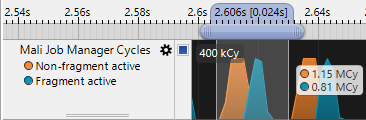
\includegraphics[width=\linewidth]{figures/khronos-wait/wait-idle.png}
\end{minipage}\hfill
\begin{minipage}[t]{.47\linewidth}\centering
\textbf{等待所需工作帧完成}\par\smallskip
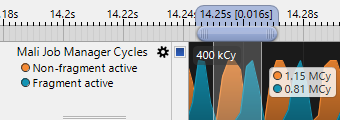
\includegraphics[width=\linewidth]{figures/khronos-wait/fences.png}
\end{minipage}
\caption{Khronos 示例中的 Arm Mali GPU 时间线，横向向右表示时间推移。橙色和蓝色表示两类 GPU 工作。左图中间有一段空白；右图按工作帧等待，后续工作能更早接上。两张原图用于读懂等待方式，Redflag 的计时另见性能册。}
\end{figure}

实时光照另有一份寿命较短的数据。切换间接光方法会重置历史计数，让新方法从第一帧开始积累；面板尺寸变化则需按新像素数建立表面与历史记录。场景中的三角形、用来加速求交的包围盒树和砖墙贴图可以继续用。退出编辑器时，先等设备空闲，移除面板的纹理登记，然后依次清理光照预览、场景与资产缓存、当前绘制设备，窗口最后释放 Vulkan 上下文。
\readings{\refitem{https://docs.vulkan.org/samples/latest/samples/performance/wait_idle/README.html}{Khronos · 等待整机与逐帧等待，原图出处}\quad
\refitem{https://docs.vulkan.org/refpages/latest/refpages/source/vkDestroyImage.html}{Vulkan · 图像销毁条件}\quad
\path{Redflag/src/Platform/Vulkan/VulkanContext.cpp}}
\endgroup
